\documentclass{article}

\usepackage[T1]{fontenc}
\usepackage[utf8]{inputenc}
\usepackage[spanish]{babel}
\usepackage{graphicx}
\usepackage{microtype}
\usepackage{xcolor}
\usepackage{amsmath}
\usepackage{amssymb}
\usepackage{mathtools}
\usepackage{xfrac}
\usepackage{booktabs}
\usepackage{hyperref}
\usepackage{siunitx}
\usepackage{float}

\newcommand{\todox}{\(\mathit{\color{red}x}\)}
\newcommand{\ham}{\large{\texttt{ham}}}
\newcommand{\spam}{\large{\texttt{spam}}}
\newcommand{\fo}{\(\mathbf{F_1}\)}

\interfootnotelinepenalty=10000

\title{Aprendizaje Automático \\ Trabajo Práctico 2 --- 4 en |}
\author{Martín Fixman \and Leandro Matayoshi \and Fernando Gasperi}
\date{Segundo Cuatrimestre de 2016}

\begin{document}
\maketitle

\newpage

\section{Introducción}

Este trabajo se propone explorar la técnica de Q Learning que permite aprender una tarea
sin necesidad de conocer ni $\delta$ (la función de transición) ni $r$ (la función de recompensa).
Analizaremos el caso concreto del juego 4 en línea para comprender cómo aprende y cómo afectan
al aprendizaje las diferentes variables que podemos controlar.

\section{Jugadores}

Modelamos el tablero y el 4 en línea de forma tal que fuera fácil simular juegos con distintos tipos de jugadores para
realizar las pruebas. Programamos 3 jugadores:
\begin{itemize}
  \item QLearn
  \item Random
  \item Minimax
\end{itemize}
El jugador Minimax tiene un horizonte de 3 jugadas y utiliza el valor 1 para los
estados ganadores, -1 para los perdedores y 0 para los de empate. Si no alcanza
una posición final mirando 3 jugadas
hacia adelante devuelve 0, el valor equivalente a un empate. Lo que podría hacer
es evaluar la posición y devolver un valor que represente el resultado de la
evaluación, es decir, cuál de los dos colores se encuentra en una posición
favorable. Sin embargo, veremos más adelante que nuestros experimentos muestran a
la evaluación innecesaria para este contexto.
El jugador Q Learning tiene varios parámetros que permiten ajustarlo:
\begin{itemize}
  \item $\epsilon$ es la probabilidad con la cual elige una acción al azar. En
    cada turno elige con probabilidad $\epsilon$ tomar una acción al azar entre
    las disponibles o tomar alguna de las que maximiza Q para el estado actual.
  \item $\alpha$ es la tasa de aprendizaje, el peso que le damos a lo aprendido
    con la nueva acción.
  \item $\gamma$ es la constante que determina el valor relativo de las
    recompensas futuras.
  \item el valor inicial de los elementos $Q_{i, j}$.
\end{itemize}
Las experimentaciones que realizaremos pretenden analizar cómo impactan estos
parámetros en el aprendizaje del jugador. Además nos interesa ver el efecto de
cuestiones externas al algoritmo como si aprende jugando sólo con un color (lo
cual decide quién comienza las partidas), con qué jugador aprende, etc.

\section{Experimentación}

\subsection{Aprendizaje}

En primera instancia nos interesa corroborar que nuestro jugador QLearn
efectivamente aprenda y logre derrotar al jugador Random. Primero pusimos a
jugar a dos jugadores Random para ver cuánto influía el hecho de que el rojo
jugara primero y si los resultados eran parejos.

\begin{figure}[H]
	\centerline{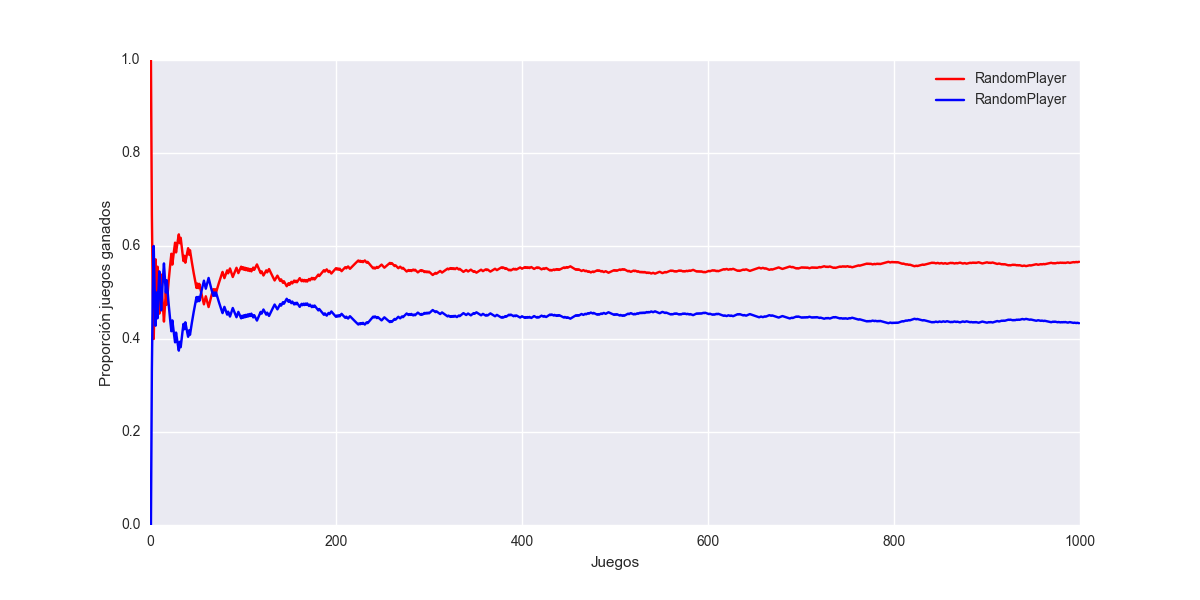
\includegraphics[width=1.3\textwidth]{figures/random_vs_random.png}}
	\caption{Random vs. Random}
\end{figure}

Jugar primero vemos que tiene una ventaja clara pero pequeña ya que la
performance de ambos se encuentra a menos de $5\%$ del empate. Ahora veamos si
QLearn puede vencer a Random. QLearn utilizará $\epsilon = 0.2$, $\alpha = 0.3$ y $\gamma = 0.9$.

\begin{figure}[H]
	\centerline{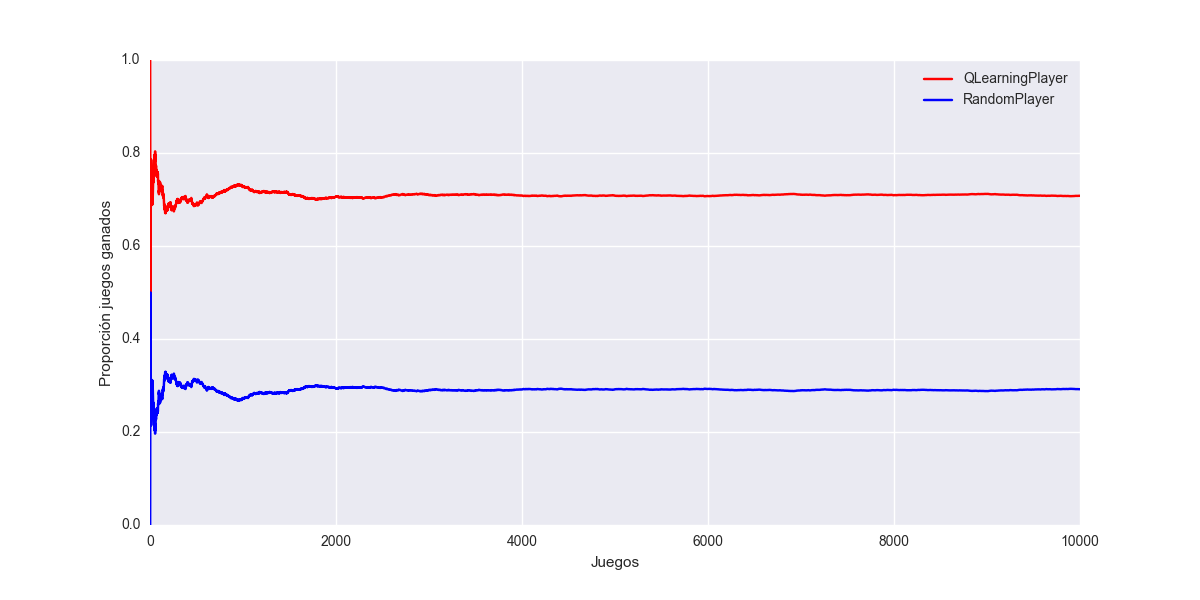
\includegraphics[width=1.3\textwidth]{figures/qlearn_vs_random.png}}
	\caption{QLearn vs. Random}
\end{figure}

QLearn logra ganarle al Random jugando primero el $70\%$ de las veces. Se puede
ver que también logra derrotar al Random jugando segundo.

\begin{figure}[H]
	\centerline{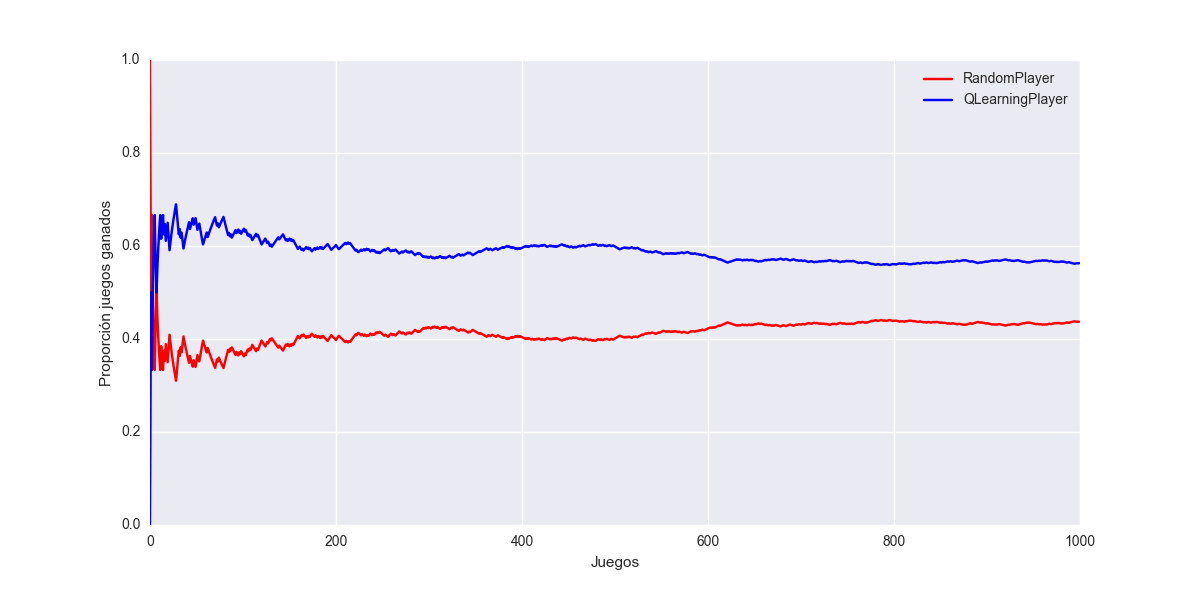
\includegraphics[width=1.3\textwidth]{figures/random_vs_qlearn.png}}
	\caption{Random vs. QLearn}
\end{figure}

Esta última es una buena muestra del desempeño de QLearn ya que logra sobrepasar
la desventaja que implica jugar segundo.

\subsection{Performance against Minimax}

Durante el TP se desarrolló una implementación de MinimaxPlayer que obtiene muy buenos resultados.
Utiliza una ventana de 3 movimientos a futuro, premiando los escenarios ganadores con un valor de 1,
castigando los escenarios perdedores con -1 y devolviendo 0 para los escenarios en donde la ventana alcanza
un valor de 0 y ningún jugador ha ganado o perdido.

Dicha implementación fue testeada contra un jugador random alcanzando un niveles de efectividad muy altos.
Debido a las características recursivas del algoritmo el algoritmo toma un tiempo no despreciable en ejecutarse,
por lo que experimentamos hasta una cantidad de juegos N con un valor máximo de 100.000

A continuación se incluye una tabla en donde mostramos la efectividad de un QLearn Player compitiendo contra
un Minimax player para distinta cantidad de juegos N.

Los parámetros del QLearn Player fueron fijados con los siguientes valores:
$\epsilon$ = 0.2, $\alpha$ = 0.3, $\gamma$ = 0.9

Los resultados están expresados en función de la cantidad de victorias del jugador QLearn sobre el total de partidos
jugados

~

\begin{center}
\begin{tabular}{c c}
	\toprule
	\textbf{\#Games} & \textbf{QLearn victories} \\
	\midrule
	0 & 0.01 \\
	1000 & 0.013 \\
	5000 & 0.0136 \\
	10000 & 0.0121 \\
	20000 & 0.01205 \\
	40000 & 0.012775 \\
	100000 & 0.0117 \\
	\bottomrule
\end{tabular}
\end{center}

~

Según los resultados podemos concluir que la cantidad de partidos jugados no son suficientes como para que el
algoritmo de QLearn desarrolle una política $\pi$ efectiva. Por el contrario, la ventana de valor 3
le es suficiente al Minimax player para poder anticipar y dirigir sus movimientos a escenarios ganadores y poder
evitar los perdedores.


\subsection{Tasa de aprendizaje}

A continuación incluimos los resultados de los experimentos en donde comparamos la forma en que el
QLearn player aprende a jugar contra distintos tipos de jugadores.

Realizamos 3 corridas diferentes, en donde variamos el rol del QLearn en el juego: Jugador
que realiza el primer movimiento, que mueve segundo o alternando los turnos de inicio.

Los parámetros del QLearn Player fueron fijados con los siguientes valores:
$\epsilon$ = 0.2, $\alpha$ = 0.3, $\gamma$ = 0.9

\begin{figure}[H]
	\centerline{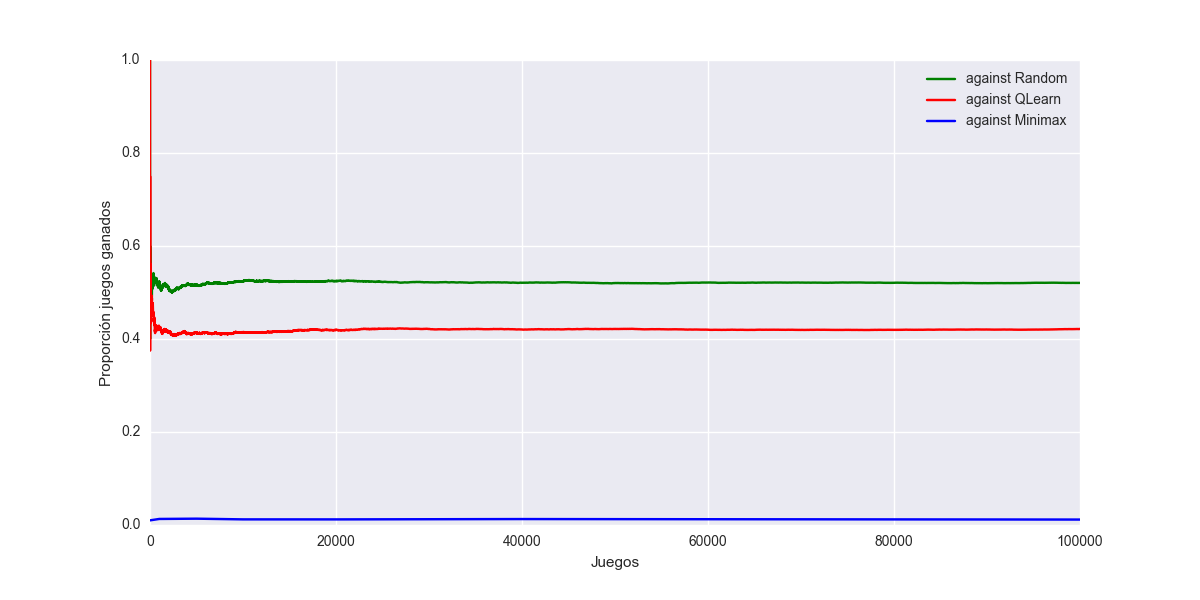
\includegraphics[width=1.3\textwidth]{figures/learning_rate_as_second_player.png}}
	\caption{Porcentaje de victorias como jugador que mueve segundo}
\end{figure}

\begin{figure}[H]
	\centerline{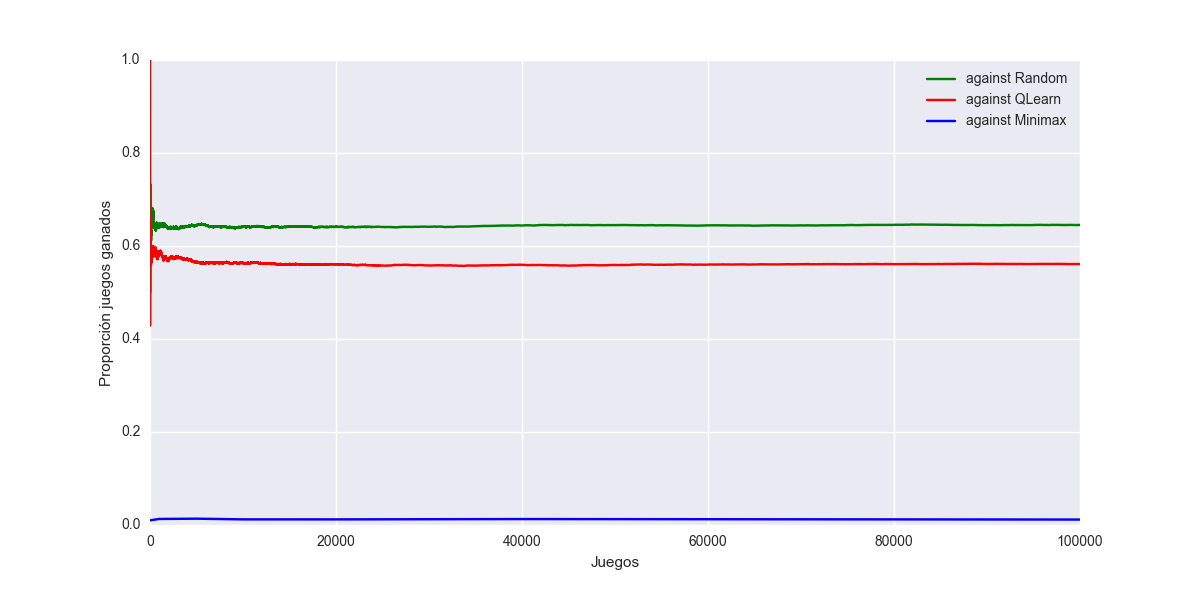
\includegraphics[width=1.3\textwidth]{figures/learning_rate_as_first_player.png}}
	\caption{Porcentaje de victorias como jugador que mueve primero}
\end{figure}

\begin{figure}[H]
	\centerline{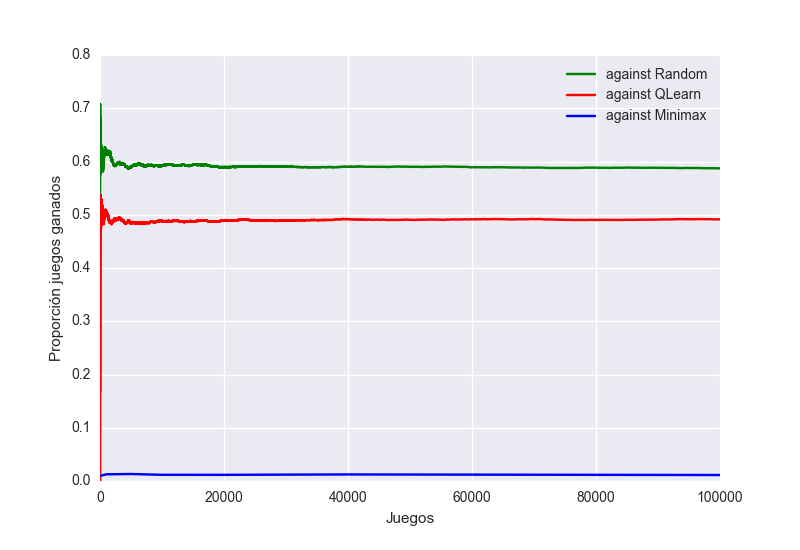
\includegraphics[width=1.3\textwidth]{figures/learning_rate_rotating_turns.png}}
	\caption{Porcentaje de victorias alternando los turnos de inicio}
\end{figure}

En los 3 casos observamos malos resultados. El porcentaje de victorias permanece constante para esa cantidad
de juegos, lo que da un indicio de que el algoritmo no obtiene mejoras inmediatas en su aprendizaje según
el tipo de jugador ni dependiendo de si empieza primero o segundo (aunque obtiene más victorias cuando
mueve primero).


\subsection{Parámetros de Q Learning}

Realizamos algunos experimentos con los parámetros de Q Learning. El objetivo de
analizar los parámetros es doble, por un lado ver cómo afectan la performance
del algoritmo y por otro encontrar los valores óptimos. Los dos parámetros
que variamos fueron $\gamma$ y $\epsilon$.

\begin{figure}[H]
	\centerline{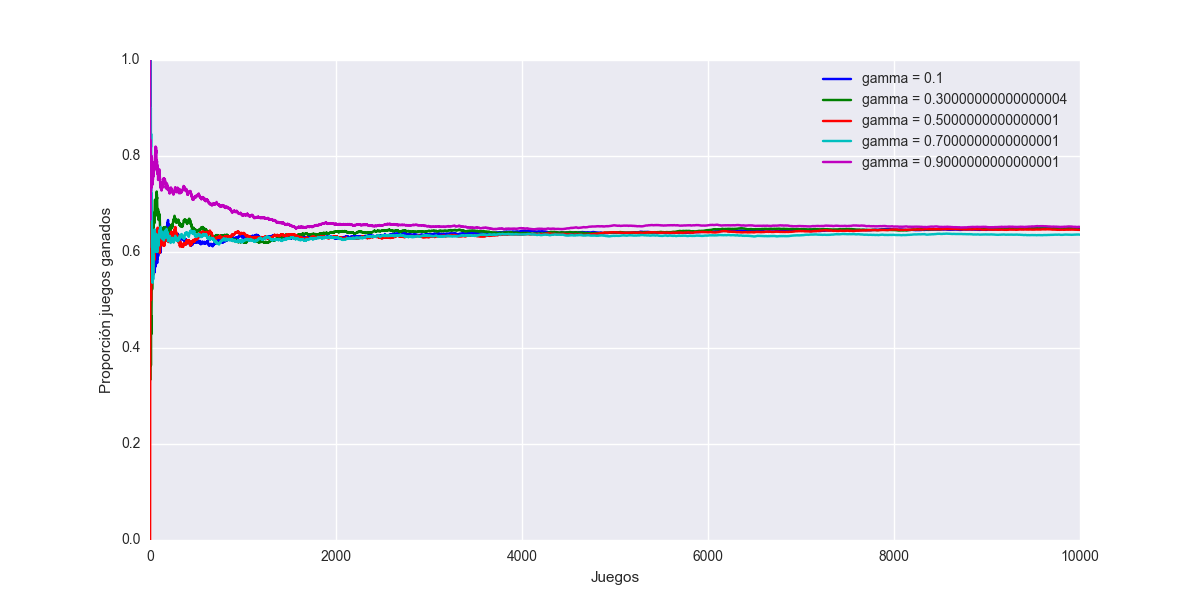
\includegraphics[width=1.3\textwidth]{figures/gamma.png}}
	\caption{Gamma}
\end{figure}

\begin{figure}[H]
	\centerline{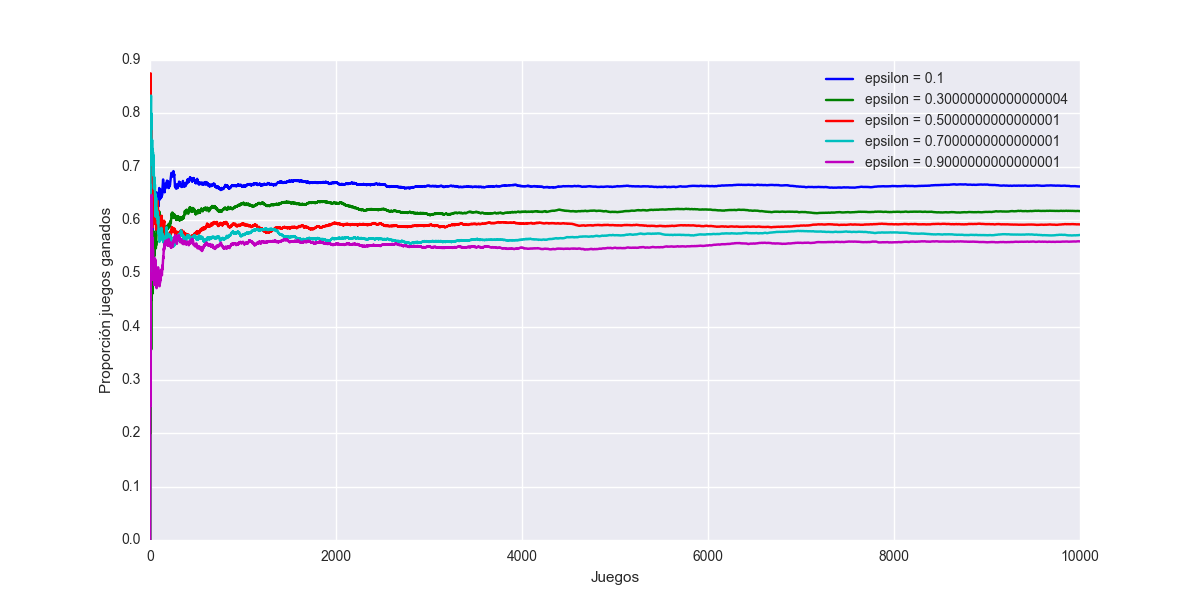
\includegraphics[width=1.3\textwidth]{figures/epsilon.png}}
	\caption{Epsilon}
\end{figure}

Se puede apreciar que $\gamma$ parece no afectar considerablemente la performance
aunque los valores superiores se encuentran favorecidos. Sin embargo, $\epsilon$
muestra un impacto mayor, consiguiendo los mejores resultados con un $\epsilon =
0.1$, el mínimo. No estamos seguros por qué un parámetro de exploración bajo
puede favorecer al algoritmo, quizás dada la reducida cantidad de partidas de
entrenamiento si se repiten posiciones que ya sabe ganar obtiene mejores
resultados en un intervalo corto pero eso no se propague a entrenamientos más largos.

\section{Conclusiones}

El algoritmo de Q Learning funciona y pudimos ver claramente que aprende ya que
consiguió vencer a otros jugadores. Queda un amplio espacio para seguir
experimentando. Nos hubiera gustado analizar el impacto del resto de los
parámetros: el valor inicial de los elementos $Q$, $\alpha$ e incluso las
distintas combinaciones que surgen de ellos. No terminamos de entender por qué
la tasa de efectividad de Q Learn no es monótona creciente, creemos que se puede
deber a que el peso de los resultados del acumulado es demasiado y tendría más
sentido tomar la tasa de efectividad de las últimas $n$ partidas en lugar del
acumulado de todas. Otra posibilidad es que el entrenamiento que realizamos fue
demasiado corto para que pueda seguir creciendo. Por último, nos hubiera gustado
comparar el resultado del aprendizaje con distintos contrincantes de alguna otra
forma, nos pareció que la tasa de efectividad como índice absoluto es pobre. Se
nos ocurrió que si hiciéramos un entrenamiento suficientemente largo como para
tener confianza en que la $Q$ obtenida se parece a la objetivo, podríamos haber
comparado las $Q$ resultantes de los entrenamientos con cada contrincante
distinto y graficar cómo progresaba la distancia a la $Q$ objetivo.

\end{document}
